\section{Visualizing charge densities and orbitals}
\label{section visualizing}

Charge densities, orbitals, etc. can be written onto a cartesian grid
in the ``cube'' file format (see below, as well as Section
\ref{section output}, specifically the \keyword{output} keyword and
the \subkeyword{output}{cube} subkeyword described there). The
visualization described in this section pertains to a simple H$_2$O
molecule, and can be repeated for example for the relaxed geometry
obtained in the relaxation testrun for H$_2$O in this distribution.

After running FHI-aims for the desired target geometry with the
appropriate output flags (see Section \ref{section output}), some
files will be generated, all of which have the extension ``*.cube". In
the H$_2$O example shown in this section, the calculation was run with
\emph{tier} 2 basis set, which should produce a more accurate charge
density, and the parameters entered in the control.in 
file were: 

\begin{verbatim}
 output cube total_density
   cube origin 0.0  0.0  0.0
   cube edge 29  0.15 0.0  0.0
   cube edge 29  0.0  0.15 0.0
   cube edge 29  0.0  0.0  0.15
 output cube eigenstate 5
 output cube eigenstate 6
\end{verbatim}

The ``Gaussian CUBE" files are written in a file format originally
defined by the ``Gaussian'' program package, but now implemented as a
\emph{de facto} standard by many visualization programs. In this
section, an example of how to visualize them using jmol program
\cite{jmol} is presented.  

The CUBE files are composed of a header and the volumetric data. The
header is divided in the following manner: 

\begin{itemize}
\item 1$^{st}$ and 2$^{nd}$ lines: text ignored by visualization programs
\item 3$^{rd}$ line:  number of atoms in the file followed by the origin around which the volumetric data will be plotted.
\item 4$^{th}$, 5$^{th}$, and 6$^{th}$ lines: number of points to be plotted, followed by the axis vector.
\item 7$^{th}$ line on, until the end of the header: one line for each atom of the system, consisting of atomic number, followed by the atom $xyz$ position.
\end{itemize}

An example of such a header with the beginning of the volumetric data is given below:

\begin{verbatim}
 CUBE FILE written by FHI-AIMS				
 *****************************
    3   -2.100000   -2.100000   -2.100000
   29    0.150000    0.000000    0.000000
   29    0.000000    0.150000    0.000000
   29    0.000000    0.000000    0.150000
    8    0.000000    0.000000    0.000000    0.000000
    1    0.000000    0.707000   -0.707000    0.000000
    1    0.000000   -0.707000   -0.707000    0.000000
  0.12810E-04  0.18208E-04  0.25394E-04  0.34819E-04  0.46974E-04  0.62322E-04
  0.81196E-04  0.10365E-03  0.12928E-03  0.15704E-03  0.18520E-03  0.21135E-03
  0.23277E-03  0.24687E-03  0.25180E-03  0.24687E-03  0.23277E-03  0.21135E-03
  .
  .
  .
\end{verbatim}

In order to visualize these files in jmol, open the program and open
the script console. Load a cube file, for example the total electronic
density, by typing the following command: 

\begin{verbatim}
> load "total_density.cube"
\end{verbatim}

This will show your molecule. In order to visualize the surfaces, one
must use the ``isosurface" command. It has a myriad of options, all of
which are explained in the jmol documentation \cite{jmol}, as of this
writing located at 
\url{http://chemapps.stolaf.edu/jmol/docs/#isosurface}. As an
example, in order to plot a volume, the command is: 

\begin{verbatim}
> isosurface cutoff <cutoff> "total_density.cube" 
\end{verbatim}

The field $<$cutoff$>$ specifies a radius for the surface, since all values equal too or less than this one will be plotted. 

Although these files are written by default in {\AA}, some programs
(including jmol), read them in atomic units (bohr) by default. In the
\emph{utilities/} folder, one can find the \texttt{angstrom\_to\_bohr.pl}
script that converts the CUBE files to atomic units. 

Plotting planes is also very easy, and the command is, for example:

\begin{verbatim}
> isosurface plane <plane_position> <other_options> "total_density.cube"
\end{verbatim}

The field $<$plane\_position$>$ can either specify the axis that
define your plane (e.g. xy) or three atoms, whose centers will specify
the plane (syntax: (atomno=1) (atomno=2) (atomno=3)). The field
$<$other\_options$>$ may contain all sorts of color scheme and/or
cutoff specifications.  

One can plot as many isosurfaces simultaneously as one wishes. The
command to delete them is simply:  

\begin{verbatim}
> isosurface delete
\end{verbatim}

Some example images and their respective commands are shown in Figure
\ref{jmol-surfaces}. The CUBE files shown were all converted to atomic
units. 

\begin{figure}[htbp]
\begin{center}
\subfigure[]{
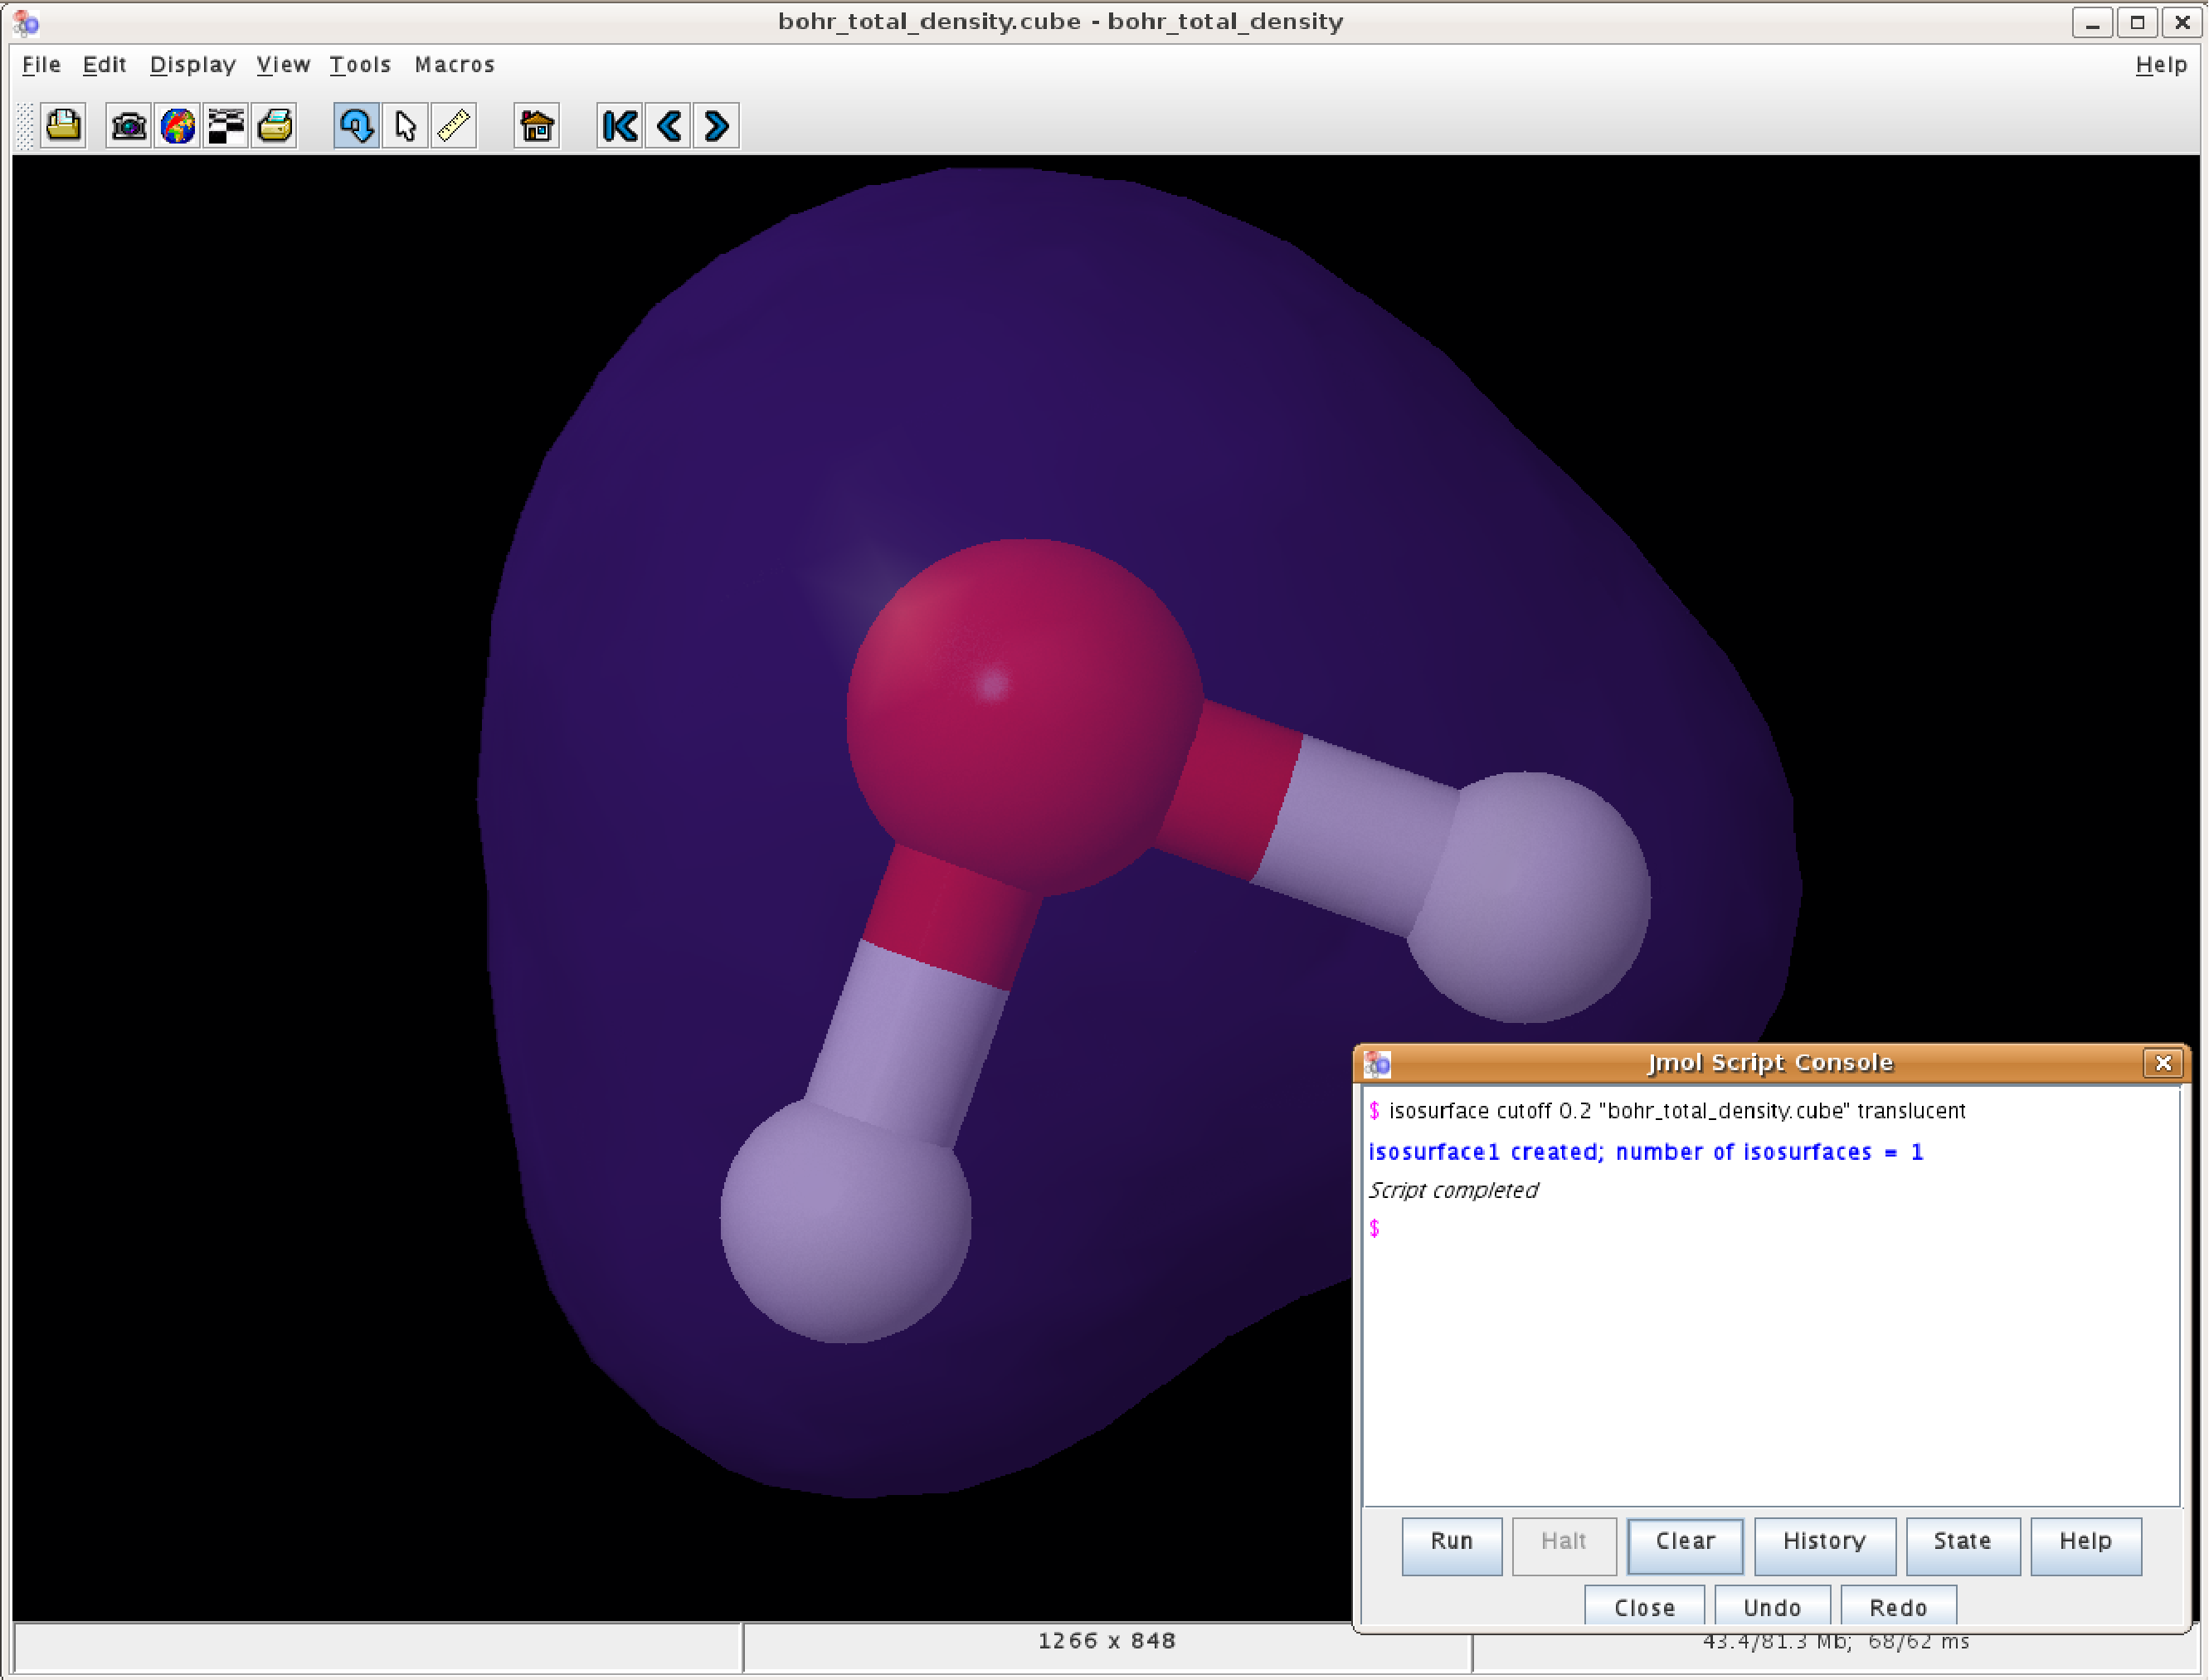
\includegraphics[height=0.21\textheight]{jmol-isosurf-1}
}
\subfigure[]{
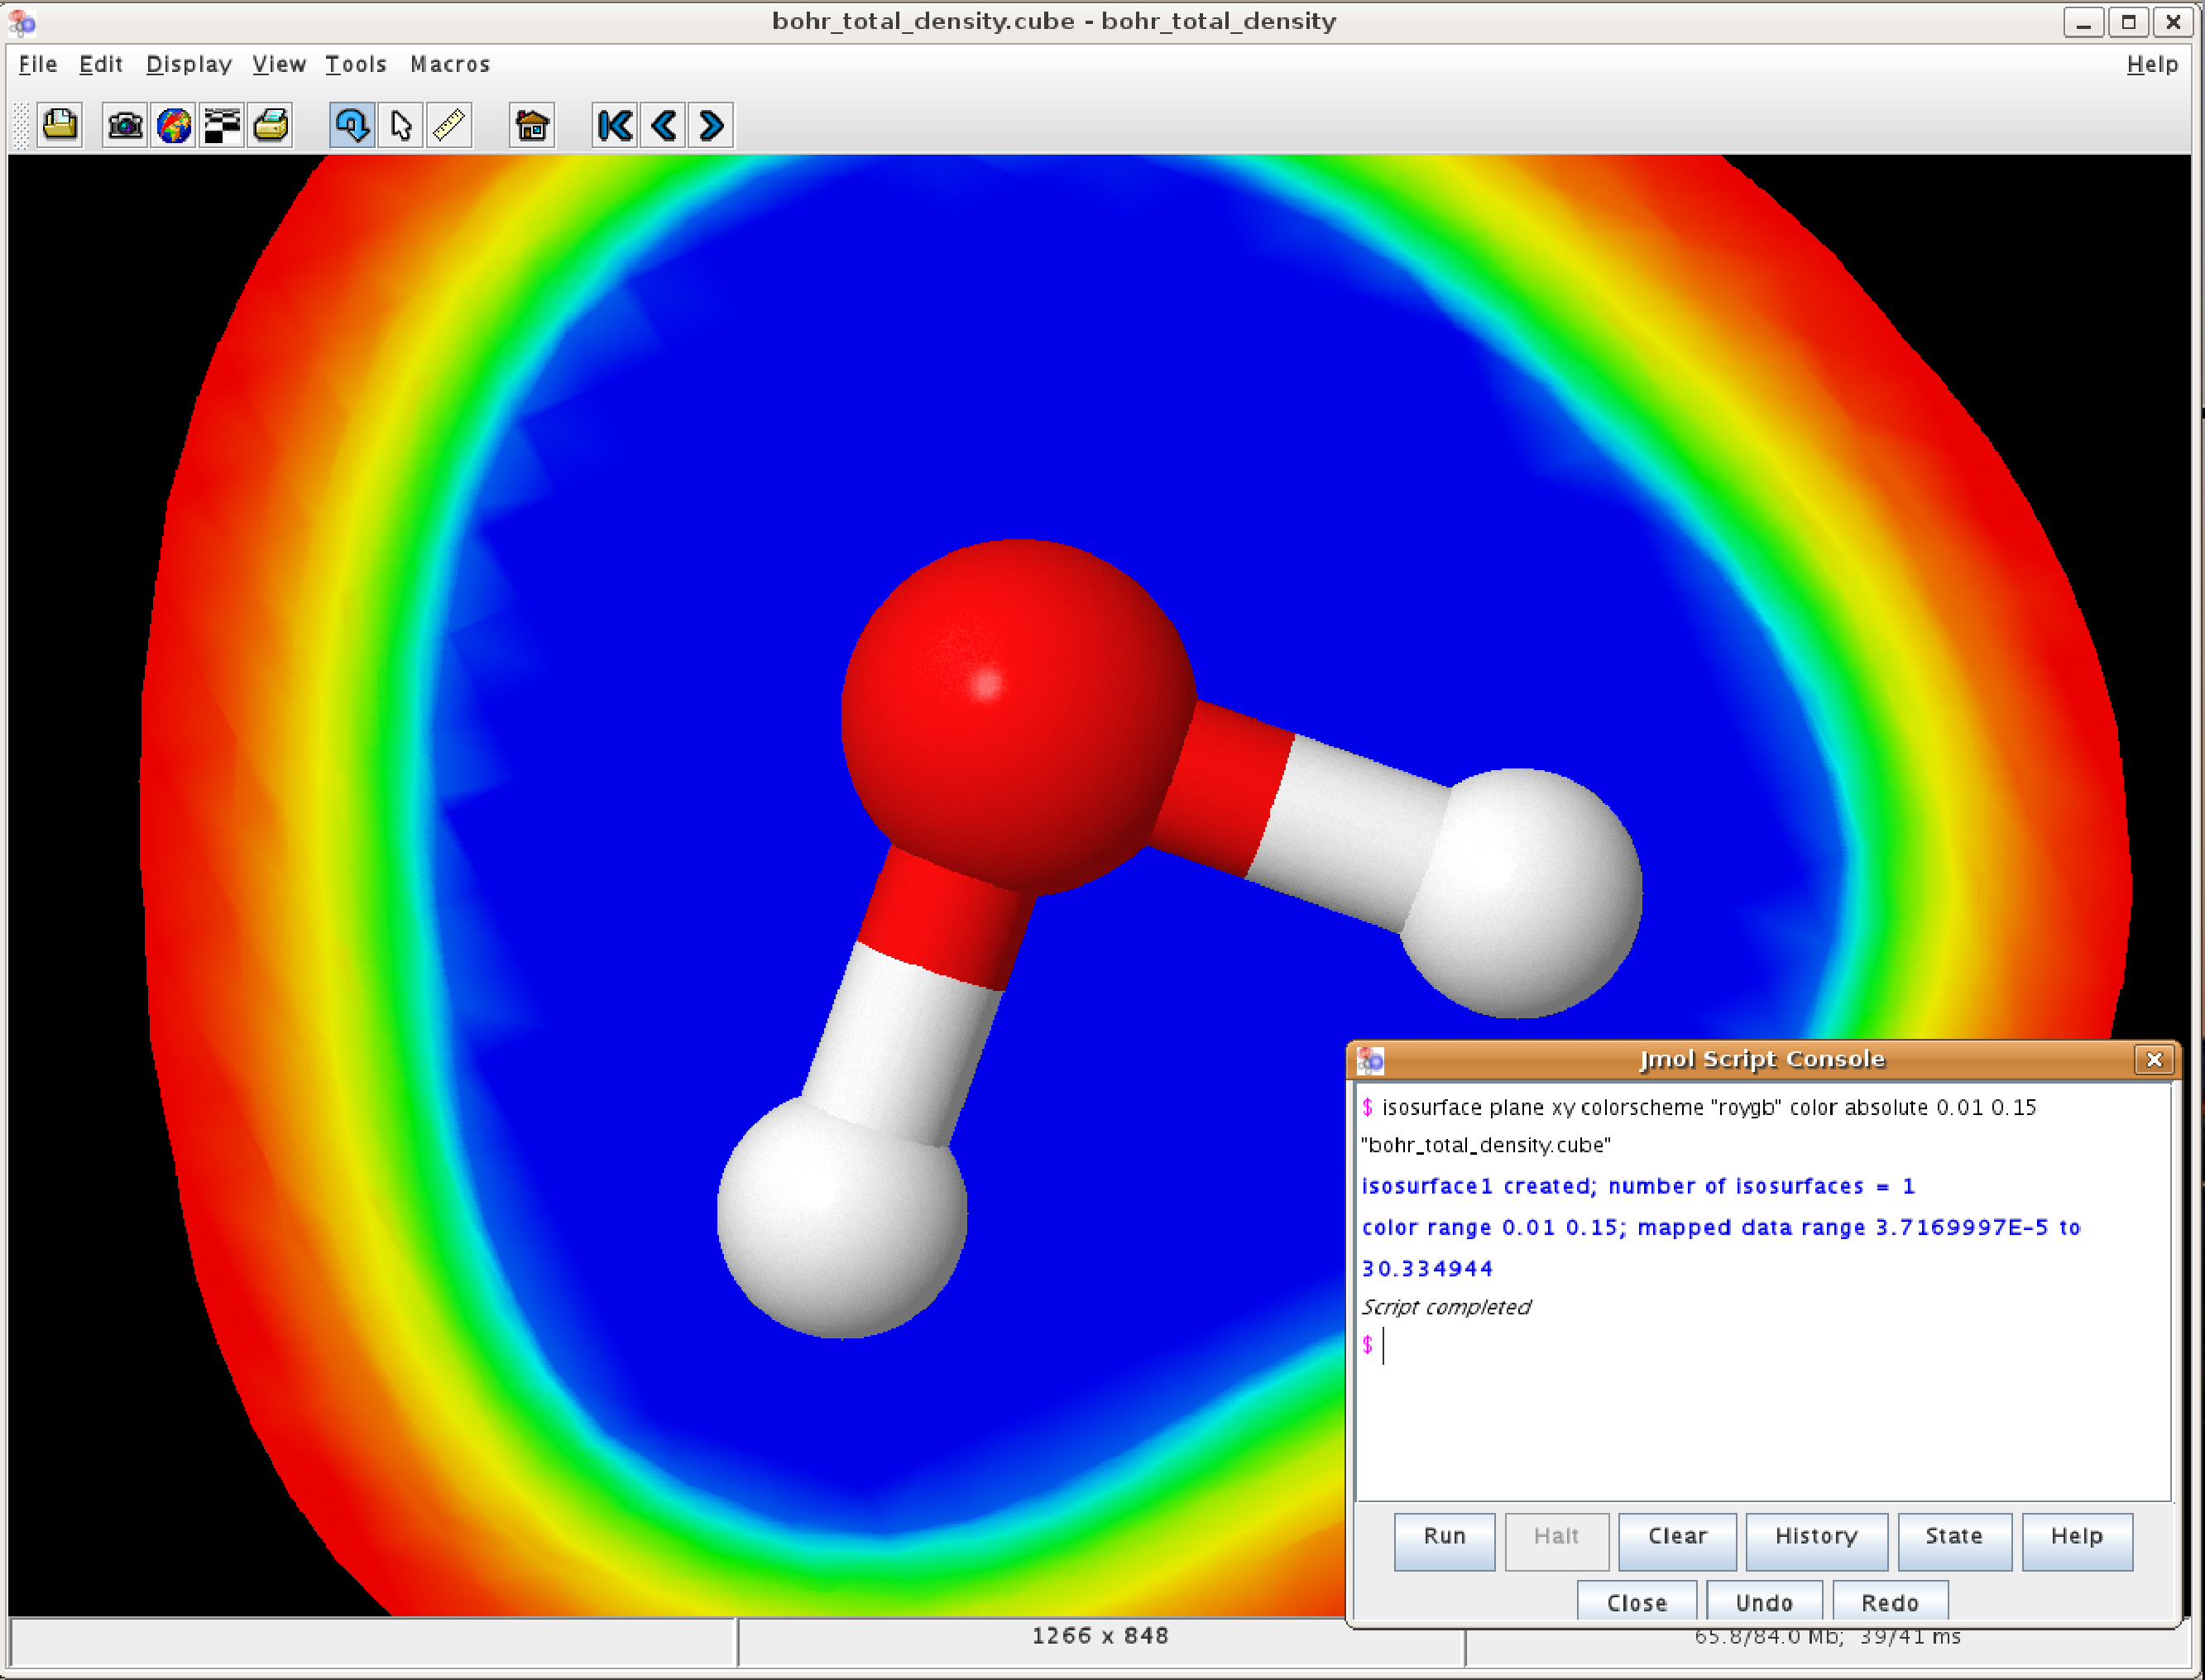
\includegraphics[height=0.21\textheight]{jmol-isosurf-2}
}
\subfigure[]{
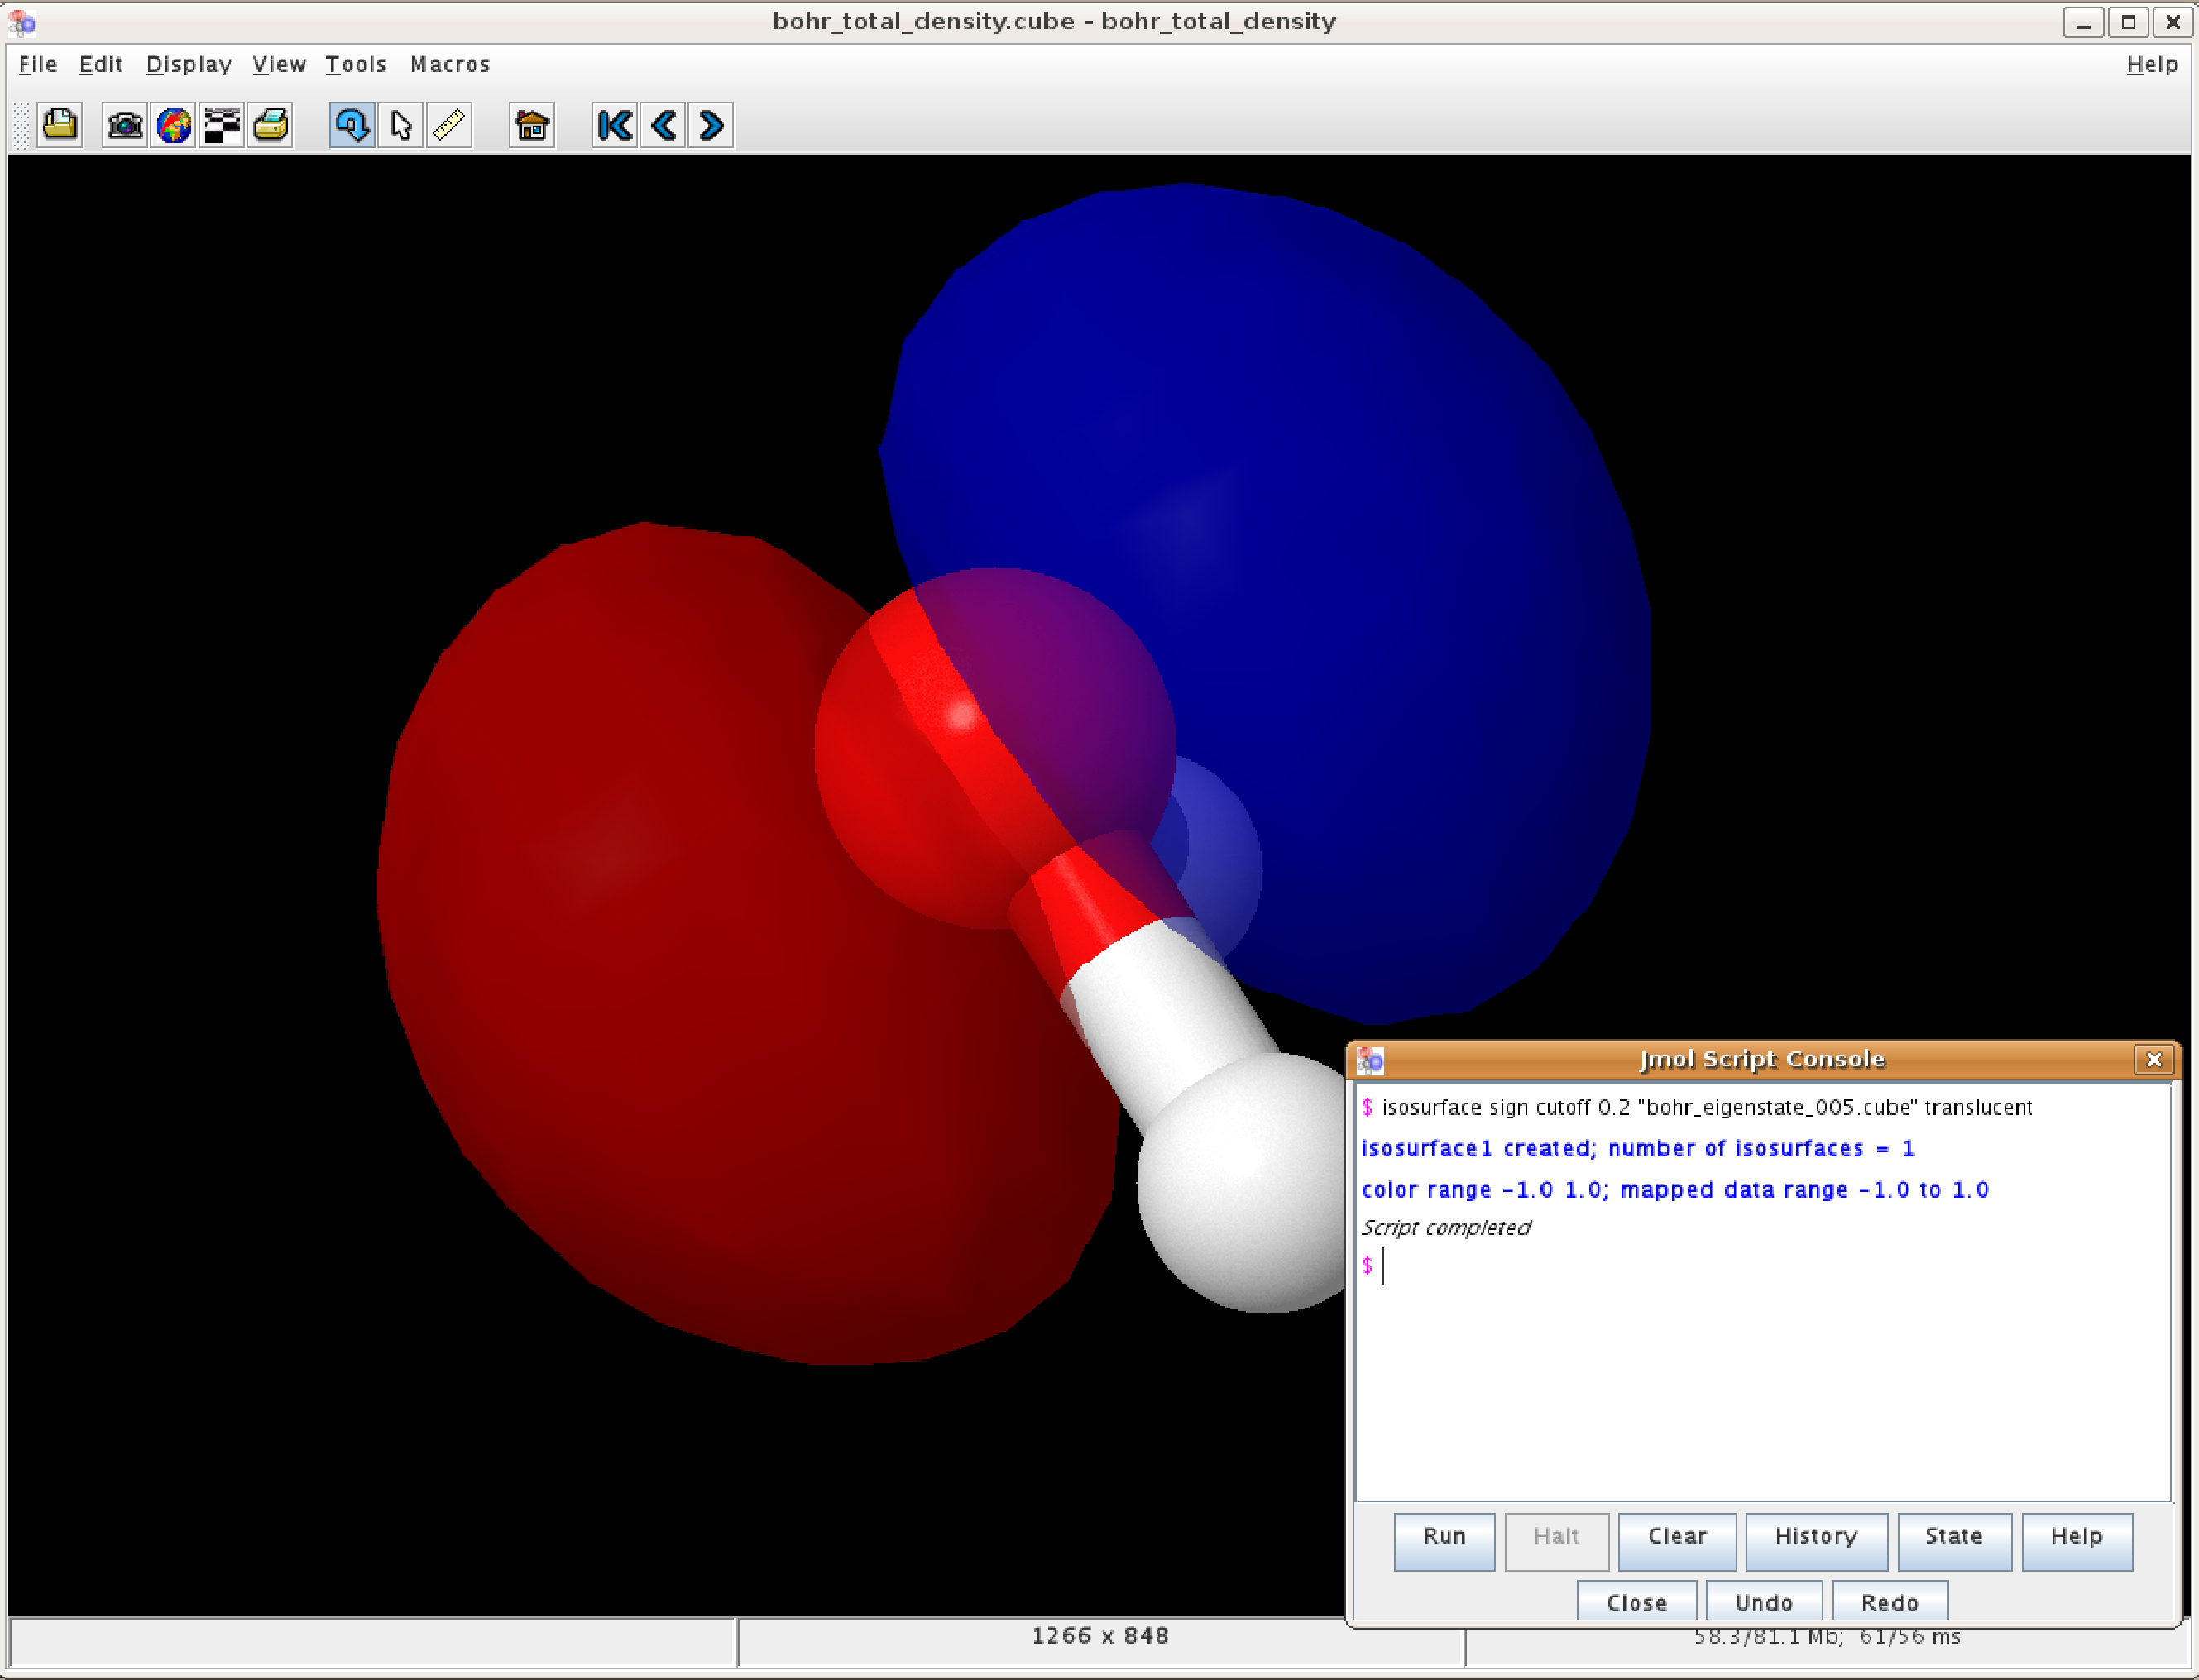
\includegraphics[height=0.21\textheight]{jmol-isosurf-3}
}
\subfigure[]{
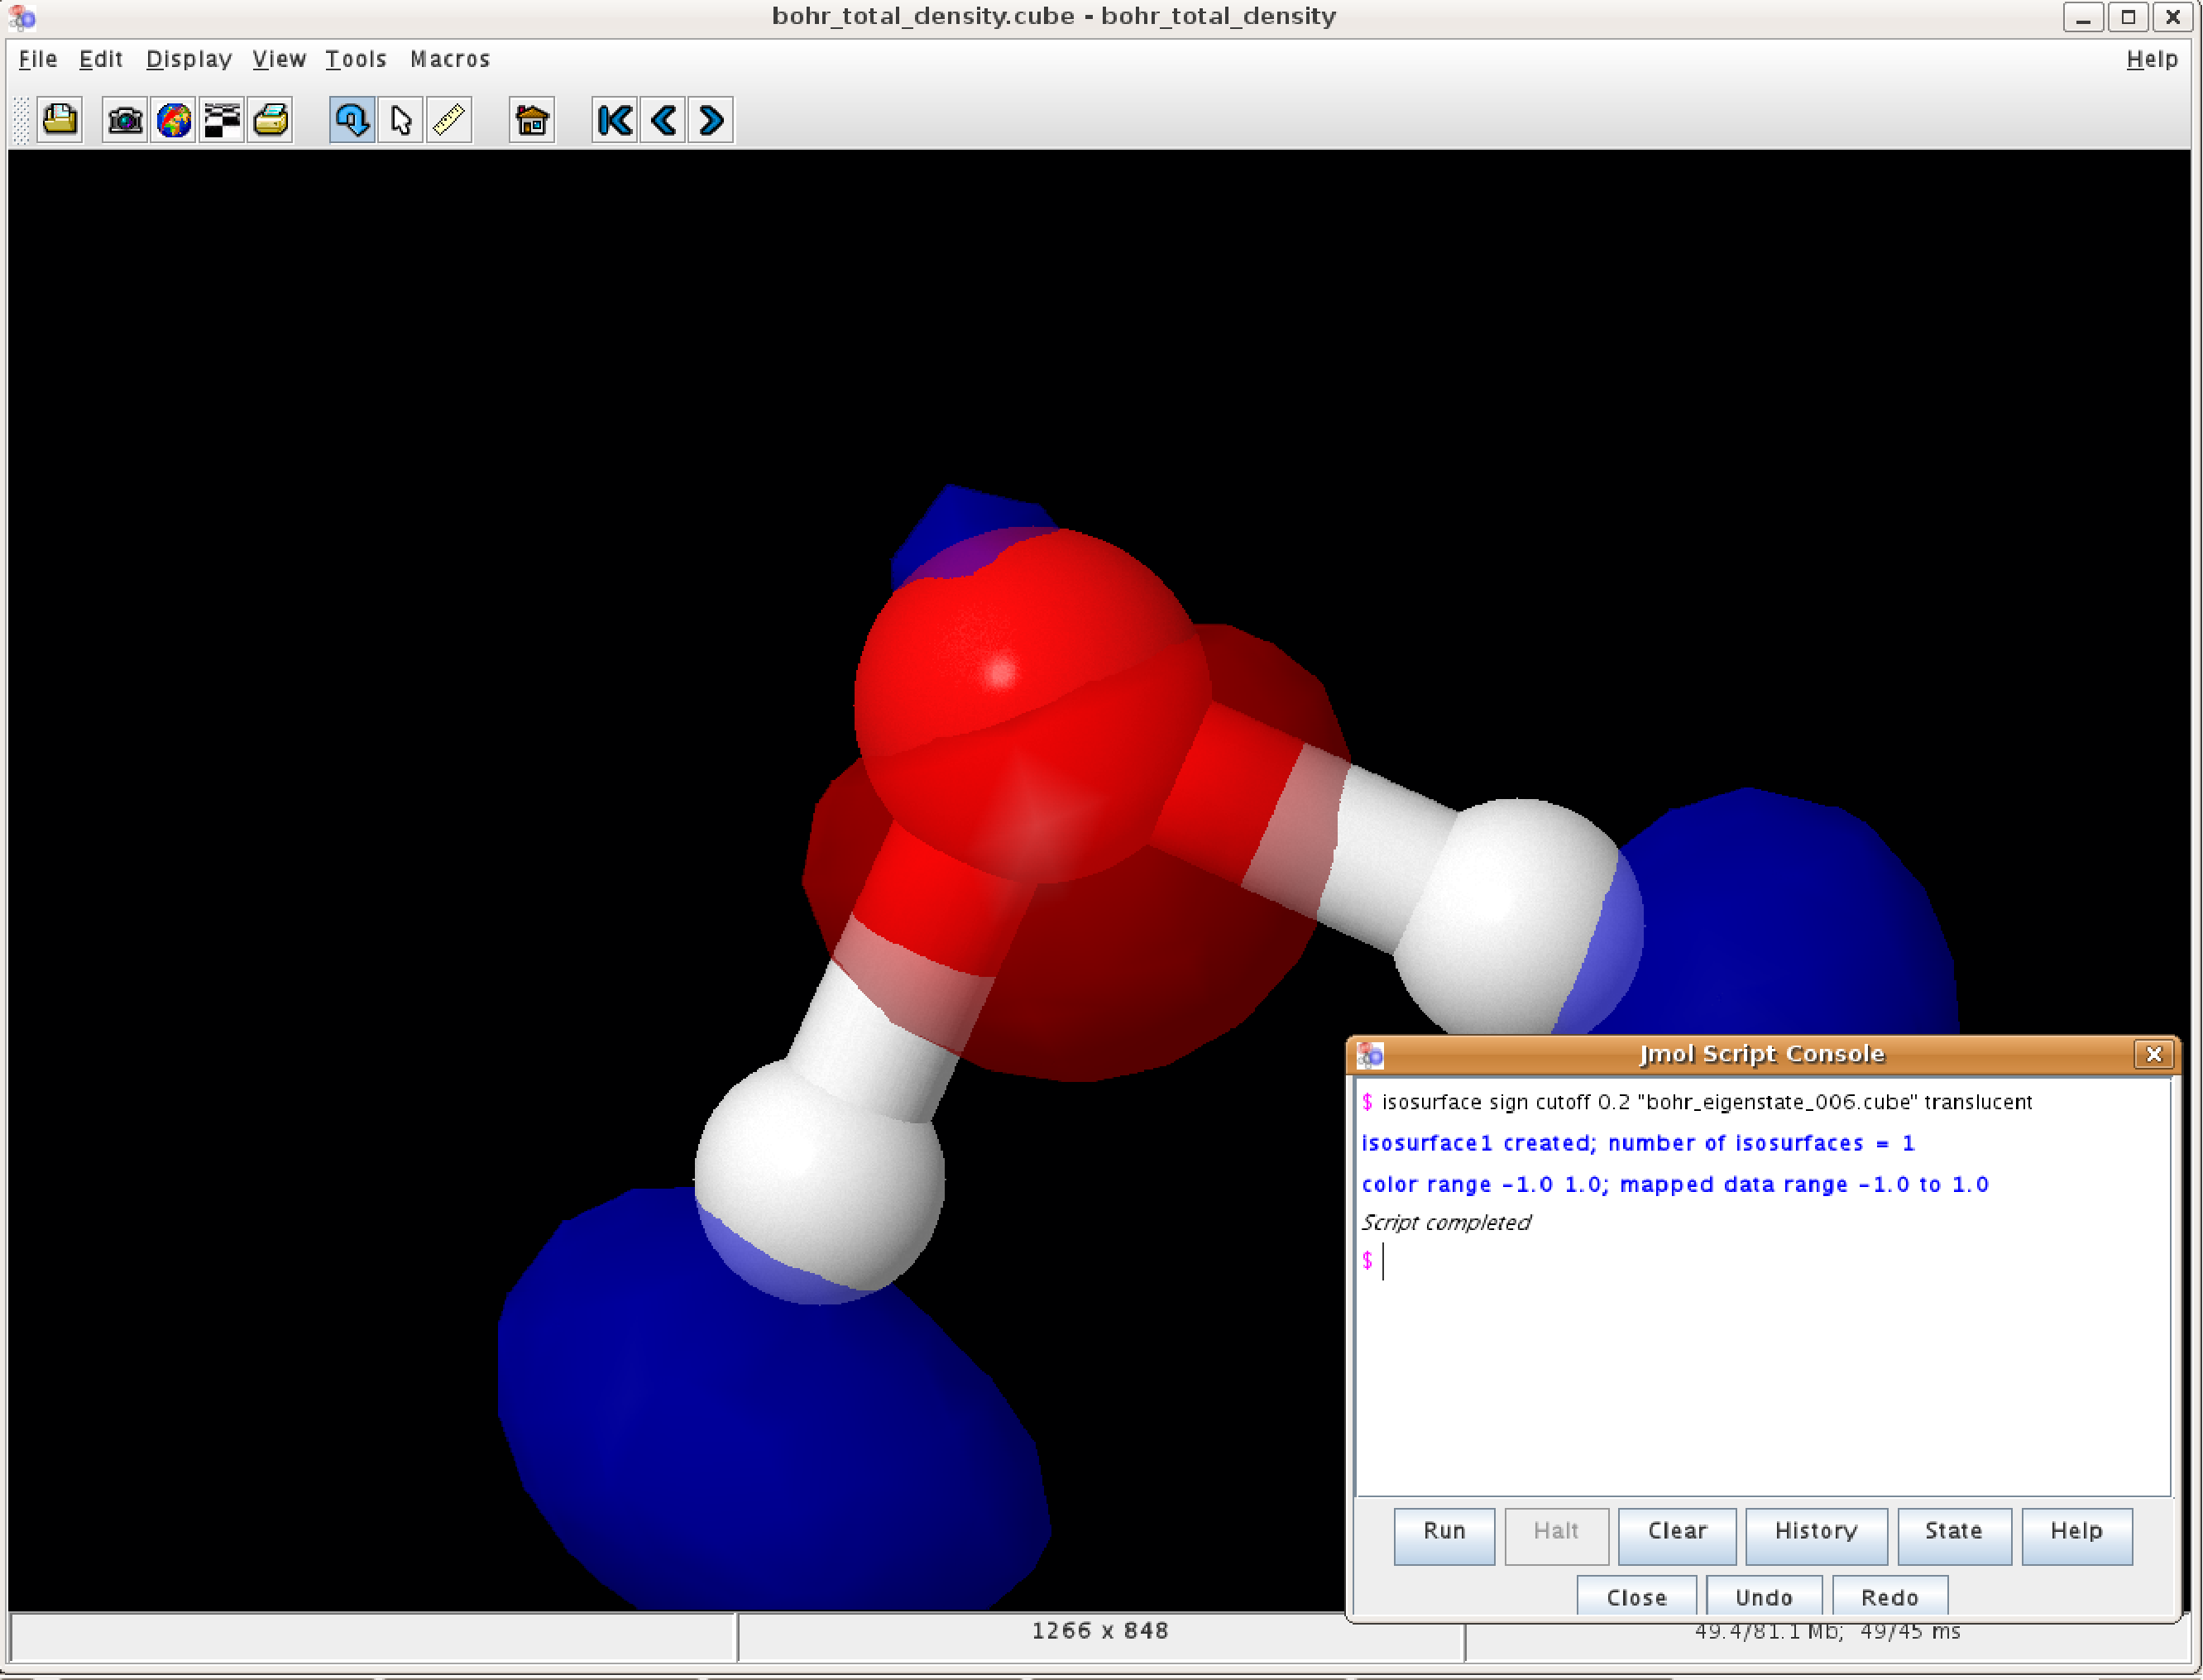
\includegraphics[height=0.21\textheight]{jmol-isosurf-4}
}
\caption{Jmol plots of charge densities and orbitals.}
\label{jmol-surfaces}
\end{center}
\end{figure}

